% Challenge dossier for Stafford's Conjecture 3.8.
% Build from this directory with:  lualatex stafford38-challenge-dossier.tex
% The listings are read from the repository files, so they cannot drift.
\providecommand{\srcroot}{../..}
\documentclass[11pt,a4paper]{article}
\usepackage[margin=2.4cm]{geometry}
\usepackage{fontspec}
\setmainfont{DejaVu Serif}
\setmonofont{DejaVu Sans Mono}[Scale=0.86]
\usepackage{amsmath,amssymb,amsthm}
\usepackage{fvextra}
\usepackage{tikz}
\usetikzlibrary{arrows.meta,positioning}
\fvset{breaklines=true,breakanywhere=true}
\usepackage[obeyspaces]{xurl}
\newcommand{\file}[1]{\path{#1}}
\usepackage{booktabs}
\usepackage{hyperref}
\hypersetup{colorlinks=true,linkcolor=blue!50!black,urlcolor=blue!50!black}
\theoremstyle{definition}
\newtheorem{definition}{Definition}
\newtheorem{convention}[definition]{Convention}
\theoremstyle{plain}
\newtheorem*{conjecture*}{Conjecture 3.8 (Stafford 1978, p.\ 438)}
\newtheorem*{theorem*}{Theorem}
\newcommand{\lean}[1]{\texttt{#1}}
\title{Stafford's Conjecture 3.8\\[0.3em]\large Challenge dossier}
\author{Christopher Albert}
\date{8 September 2026}
\begin{document}
\maketitle

\noindent
This dossier fixes the meaning of every symbol before it is used. Section 1
defines the objects in the words of the manuscript. Section 2 quotes the
conjecture and states the theorem. Section 3 defines every Lean and Mathlib
construction that the challenge file uses, then lists the file. Section 4
does the same for the solution file. Section 5 lists the second, exact-source
Challenge and its Solution. Section 6 is a clickable map of the imported
proof architecture. Section 7 records how the pairs are checked.

\section{The objects, as defined in the manuscript}

\begin{convention}[Field]
Throughout, $k$ is a field of characteristic zero: a commutative ring in which
every nonzero element is invertible and in which $1+1+\dots+1$ is never $0$.
Examples are $\mathbb{Q}$, $\mathbb{R}$, $\mathbb{C}$, and every subfield of
$\mathbb{C}$. No algebraic closure is assumed.
\end{convention}

\begin{definition}[Weyl algebra]
For $n\ge 0$, the $n$th Weyl algebra over $k$ is the associative unital
$k$-algebra
\[
  A_n=A_n(k)=k\langle x_1,\dots,x_n,\partial_1,\dots,\partial_n\rangle
\]
generated by $2n$ symbols subject to the relations
\[
  [\partial_i,x_j]=\delta_{ij},\qquad [x_i,x_j]=[\partial_i,\partial_j]=0,
\]
where $[a,b]=ab-ba$ and $\delta_{ij}$ is $1$ for $i=j$ and $0$ otherwise. It is
the algebra of polynomial-coefficient differential operators on
$k[x_1,\dots,x_n]$, with $\partial_i$ acting as $\partial/\partial x_i$. For
$n=0$ it is the field $k$ itself. It is noncommutative for $n\ge 1$; it has no
zero divisors, and its only units are the nonzero scalars.
\end{definition}

\begin{convention}[Sides and written order]
All ideals of Weyl algebras are right ideals, and all modules are right
modules. For $a\in A_n$ the right ideal generated by $a$ is
$aA_n=\{ac : c\in A_n\}$, with the cofactor on the right. Every identity is
read in the order in which its factors are written: a membership $a\in bA_n$
means $a=bc$ with $c$ on the right. No statement here is invariant under
silently transposing a product.
\end{convention}

\begin{definition}[Sum of two right ideals, and membership of $1$]
For $d,f\in A_n$, the sum $dA_n+fdA_n$ is the right ideal
$\{dR+fdS : R,S\in A_n\}$. It equals $A_n$ if and only if it contains $1$,
that is, if and only if there are $R,S\in A_n$ with
\[
  1=dR+fdS .
\]
The element $f$ stands to the left of $d$ in the second summand; $R$ and $S$
stand to the right.
\end{definition}

\begin{definition}[Bernstein filtration and Bernstein degree]
The Bernstein filtration of $A_n$ assigns degree $1$ to every generator $x_i$
and every $\partial_i$; its $m$th step is spanned by the products of at most
$m$ generators. Its associated graded ring is the commutative polynomial ring
$k[x_1,\dots,x_n,\xi_1,\dots,\xi_n]$ in $2n$ variables, where $\xi_i$ is the
image of $\partial_i$. The Bernstein degree $\deg_B d$ of a nonzero $d$ is the
smallest $m$ with $d$ in the $m$th step. In the normal form of $d$ as a
$k$-linear combination of ordered monomials $x^\alpha\partial^\beta$, it is the
maximum of $|\alpha|+|\beta|$ over the monomials that occur. It is $0$ exactly
for nonzero scalars.
\end{definition}

\begin{definition}[Linear symplectic change of generators, linear Weyl coordinate]
The $k$-span $V$ of the $2n$ generators carries the alternating bilinear form
$\omega(u,v)=[u,v]\in k$. A linear symplectic change of generators is a
$k$-linear automorphism $g$ of $V$ with $\omega(gu,gv)=\omega(u,v)$; it extends
uniquely to a $k$-algebra automorphism of $A_n$, because it preserves the
defining relations. A linear Weyl coordinate is an element
$\ell=g(x_1)\in V$ for such a $g$: a $k$-linear combination of the generators
that can serve as the first coordinate of a new set of generators satisfying
the Weyl relations. Equivalently, $\ell$ is any nonzero element of $V$, since
every nonzero vector of a symplectic space extends to a symplectic basis.
\end{definition}

\section{The conjecture and the theorem}

J.\ T.\ Stafford, \emph{Module structure of Weyl algebras}, Journal of the
London Mathematical Society (2) \textbf{18} (1978), 429--442, states on
page 438:

\begin{conjecture*}
Let $d\in A_n$. Then there exists $f\in A_n$ such that $A_n=dA_n+fdA_n$.
\end{conjecture*}

This is the complete printed statement, verified against the primary source
on 2026-09-05. By the definitions above it says: there are $f,R,S\in A_n$ with
$1=dR+fdS$. The printed sentence has no hypothesis on $d$. For $d=0$ the
right-hand side is the zero ideal, so the statement as printed is false for
$d=0$. The paragraph that follows it in the article checks the conjecture for
$n=1$ and for monomial $d$, and its equivalence argument takes $d\ne 0$
explicitly. The intended statement is the one for nonzero $d$, and that is the
statement of the theorem and of the challenge. The manuscript records this in a
footnote instead of altering the quotation.

Bellamy's 2026 survey (\emph{Module structure of Weyl algebras}, J.\ London
Math.\ Soc.\ \textbf{113} (2026), e70373, Section 3, Conjecture 3.4) states the
weaker form that every finitely generated torsion $A_n$-module is cyclic, notes
that Stafford's formulation is stronger, and reports the problem as open.

\begin{theorem*}[manuscript, Theorem 1]
For every characteristic-zero field $k$, every $n\ge 1$, and every nonzero
$d\in A_n(k)$, there exist $F,R,S\in A_n(k)$ such that
\[ 1 = dR + FdS. \]
Moreover one may choose $F=\ell^{\deg_B d}$ for a linear Weyl coordinate
$\ell$, obtained by an invertible linear symplectic change of generators.
\end{theorem*}

The first sentence is the conjecture for nonzero $d$. The second sentence is
the exact-degree strengthening: the multiplier can be taken to be a power of a
single linear Weyl coordinate, and the exponent is the Bernstein degree of
$d$. Both sentences are proved in Lean from Mathlib. The challenge below
states the first sentence; the separate exact-source Challenge in Section~\ref{sec:fixed-source} states the strengthening. The original Challenge includes $n=0$, where a nonzero $d$ is a unit
and one may take $R=d^{-1}$, $F=S=0$.

\section{The challenge}

\subsection{The Lean and Mathlib constructions used}

The challenge file uses the following constructions. The descriptions of the
Mathlib items are the docstrings of the pinned Mathlib revision.

\begin{description}\sloppy
\item[\lean{Type*}] A universe-polymorphic type. Quantifying over
  \lean{k : Type*} means the statement holds for a field of any size.
\item[\lean{Field k}] Mathlib's field structure on \lean{k}: a commutative
  ring with $0\ne 1$ in which every nonzero element has an inverse.
\item[\lean{CharZero k}] Mathlib's class: the map $\mathbb{N}\to k$,
  $m\mapsto 1+\dots+1$ ($m$ times), is injective. This is characteristic zero.
\item[\lean{$\mathbb{N}$}] The natural numbers $0,1,2,\dots$
\item[\lean{Fin n}] The type of natural numbers below \lean{n}, that is
  $\{0,\dots,n-1\}$. It has exactly $n$ elements.
\item[\lean{$\alpha$ $\oplus$ $\beta$}] The disjoint union (sum type) of two
  types. Its elements are \lean{Sum.inl a} for $a$ in $\alpha$ and
  \lean{Sum.inr b} for $b$ in $\beta$.
\item[\lean{Matrix $\iota$ $\iota$ k}] Functions $\iota\times\iota\to k$, that is
  square matrices indexed by $\iota$ with entries in $k$.
\item[\lean{Matrix.J l R}] ``The matrix defining the canonical skew-symmetric
  bilinear form.'' It is defined in \lean{Mathlib.LinearAlgebra.SymplecticGroup}
  as \lean{Matrix.fromBlocks 0 (-1) 1 0}: on the index set
  $l\oplus l$ the block $(\mathrm{inl},\mathrm{inr})$ is $-1$, the block
  $(\mathrm{inr},\mathrm{inl})$ is $+1$, and the diagonal blocks are $0$.
\item[\lean{FreeAlgebra k X}] ``Given a commutative semiring \lean{R}, and a
  type \lean{X}, we construct the free unital, associative \lean{R}-algebra on
  \lean{X}. One can think of \lean{FreeAlgebra R X} as the free
  non-commutative polynomial ring with coefficients in \lean{R} and variables
  indexed by \lean{X}.'' With $X$ the generator set, this is
  $k\langle x_1,\dots,x_n,\partial_1,\dots,\partial_n\rangle$ before any
  relation is imposed.
\item[\lean{FreeAlgebra.$\iota$ k}] ``The canonical function
  \lean{X → FreeAlgebra R X}'': it sends an index to the corresponding
  generator.
\item[\lean{algebraMap k A}] The structure map $k\to A$ of a $k$-algebra $A$,
  sending a scalar to the corresponding constant.
\item[\lean{RingQuot r}] ``The quotient of a ring by an arbitrary relation.''
  For a relation \lean{r} on a ring, \lean{RingQuot r} is the quotient by the
  smallest two-sided ring congruence containing \lean{r}. When the ring is a
  $k$-algebra, the quotient is again a $k$-algebra.
\item[\lean{def}, \lean{abbrev}] A definition; \lean{abbrev} marks it as
  transparent to Lean's unifier, so that \lean{WeylAlg k n} and its unfolding
  are interchangeable.
\item[\lean{Prop}] The type of propositions. A term of type \lean{P : Prop}
  is a proof of \lean{P}.
\item[\lean{∀}, \lean{∃}, \lean{→}, \lean{≠}] For all, there exists,
  implication, and inequality.
\item[\lean{theorem ... := by sorry}] A theorem whose proof is left open.
  \lean{sorry} is the placeholder; Lean records any theorem depending on it as
  depending on the axiom \lean{sorryAx}. In a challenge file it marks the hole
  that a solution must fill.
\end{description}

\subsection{The file}

\VerbatimInput[fontsize=\small,frame=single,label=Challenge.lean]{\srcroot/Challenge.lean}

\subsection{Correspondence with Section 1}

\begin{center}
\begin{tabular}{@{}lp{9.2cm}@{}}
\toprule
Lean & Manuscript \\
\midrule
\lean{PhaseVar n} & The index set of the $2n$ generators. \lean{Sum.inl i} is
  $x_{i+1}$ and \lean{Sum.inr i} is $\partial_{i+1}$ (indices in \lean{Fin n}
  start at $0$). \\
\lean{relation (Matrix.J (Fin n) k)} & The Weyl relations. For
  $i=\mathrm{inr}\,a$, $j=\mathrm{inl}\,b$ the entry of $J$ is $\delta_{ab}$,
  giving $\partial_a x_b-x_b\partial_a=\delta_{ab}$; for $i=\mathrm{inl}\,a$,
  $j=\mathrm{inr}\,b$ it is $-\delta_{ab}$, the same relation with the sides
  exchanged; the diagonal blocks give $[x_a,x_b]=[\partial_a,\partial_b]=0$. \\
\lean{WeylAlg k n} & $A_n(k)$: the free algebra modulo those relations. \\
\lean{d ≠ 0} & The nonzero hypothesis discussed in Section 2. \\
\lean{1 = d * R + F * d * S} & The identity $1=dR+FdS$, in the algebra
  product, with the factors in the written order. \\
\lean{UniversalStatement} & The conjecture for nonzero $d$, over every
  characteristic-zero field and every $n\ge 0$. \\
\bottomrule
\end{tabular}
\end{center}

\section{The solution}

\subsection{The additional constructions used}

\begin{description}\sloppy
\item[\lean{Stafford38.FoundationClosure}] The module of the substantive
  development that exports the proved theorem
  \lean{Stafford38.universalStatement : Stafford38.UniversalStatement}. Its
  proof uses only the axioms \lean{propext}, \lean{Classical.choice}, and
  \lean{Quot.sound}.
\item[\lean{Stafford38.WeylAlg k n}] The substantive development's Weyl
  algebra, defined in \lean{Stafford38/Statement.lean} as
  \lean{Stafford.FreeWeyl k (Fin n ⊕ Fin n) (Matrix.J (Fin n) k)}, where
  \lean{Stafford.FreeWeyl k ι omega} is
  \lean{RingQuot (freeWeylRelation omega)} and \lean{freeWeylRelation} has the
  same defining expression as \lean{relation} above. Hence
  \lean{Stafford38.WeylAlg k n} and the challenge's \lean{WeylAlg k n} are the
  same type by unfolding definitions.
\item[\lean{Stafford38.UniversalStatement}] The same proposition as
  \lean{UniversalStatement}, stated on \lean{Stafford38.WeylAlg}.
\item[\lean{A ≃ₐ[k] B}] A $k$-algebra isomorphism between $A$ and $B$
  (Mathlib's \lean{AlgEquiv}). \lean{AlgEquiv.refl} is the identity
  isomorphism of an algebra with itself; Lean accepts it here only because the
  two types are definitionally equal.
\item[\lean{e.injective}, \lean{e.symm}] An isomorphism is injective, and
  \lean{e.symm} is its inverse.
\item[\lean{intro}, \lean{rcases}, \lean{refine}, \lean{simpa}, \lean{congrArg}]
  Tactic steps: introduce the quantified variables; destructure the existential
  witnesses $F,R,S$ and the identity from the substantive theorem; supply the
  witnesses of the goal; and close the remaining equality by applying
  \lean{e.symm} to both sides of the known identity and simplifying, using that
  \lean{e.symm} is an algebra map and so preserves $1$, sums, and products in
  their order.
\end{description}

\subsection{The file}

\VerbatimInput[fontsize=\small,frame=single,label=Solution.lean]{\srcroot/Solution.lean}

\begin{sloppypar}
The solution repeats the challenge definitions verbatim, so its
\lean{UniversalStatement} has exactly the challenge's type; the comparison in
Section 5 checks this mechanically. The proof transports the substantive
theorem along the identity isomorphism and returns the witnesses. No
hypothesis is added and no factor is moved.
\end{sloppypar}


\section{The exact-source Challenge}\label{sec:fixed-source}

The original pair asks for an arbitrary multiplier $F$. The new pair asks for
$F=\ell^{\deg_B d}$, with $\ell$ a linear symplectic coordinate and $n\ge1$.
The Challenge imports only Mathlib and presents the Weyl algebra exactly as
in Section 3. Its degree is intrinsic to the presented element: $\deg_B d$ is
the least $N$ such that $d$ lies in the $k$-span of the images of the ordered
words $x^{a}\partial^{p}$ with $|a|+|p|\le N$, where the ordered words are
built recursively from the generators in the free algebra. The coordinate
$\ell$ is the first coordinate of an invertible linear symplectic change of
the generators, given by matrices $M$, $N$ with $MJM^{\mathsf T}=J$,
$NJN^{\mathsf T}=J$, $MN=NM=1$. Neither a degree, nor a normal form, nor an
equivalence is supplied as a hypothesis; the file below is the whole
statement. The transport module
\file{Stafford38/FixedSourceChallengeTransport.lean} repeats these
definitions without importing the Challenge and proves that the intrinsic
filtration is the development's Bernstein filtration and that its least level
is the checked PBW normal-form degree; the two coordinate predicates are
definitionally equal. The Solution combines that with the proved theorem. The
consumer file \file{tests/FixedSourceChallengeConsumer.lean} evaluates the
intrinsic degree at the unit ($0$, once without the transport) and at a
coordinate ($1$), and instantiates the compared theorem at both.

\VerbatimInput[fontsize=\scriptsize,frame=single,label=FixedSourceChallenge.lean]{\srcroot/FixedSourceChallenge.lean}
\VerbatimInput[fontsize=\small,frame=single,label=FixedSourceSolution.lean]{\srcroot/FixedSourceSolution.lean}
\VerbatimInput[fontsize=\small,frame=single,label=comparator-fixed-source.json]{\srcroot/comparator-fixed-source.json}

\section{Architecture of the imported proof}\label{sec:architecture}
\hyperref[sec:literature]{Literature and source roles for this map}.

The arrows below point from a prerequisite to the step that uses it. Each
box links to its explanation. This is a summary of the terminal route in
\texttt{docs/proof-graph.yaml}; the separately checked tangent-limit lemma is
auxiliary and has no edge into this route.

\begin{center}
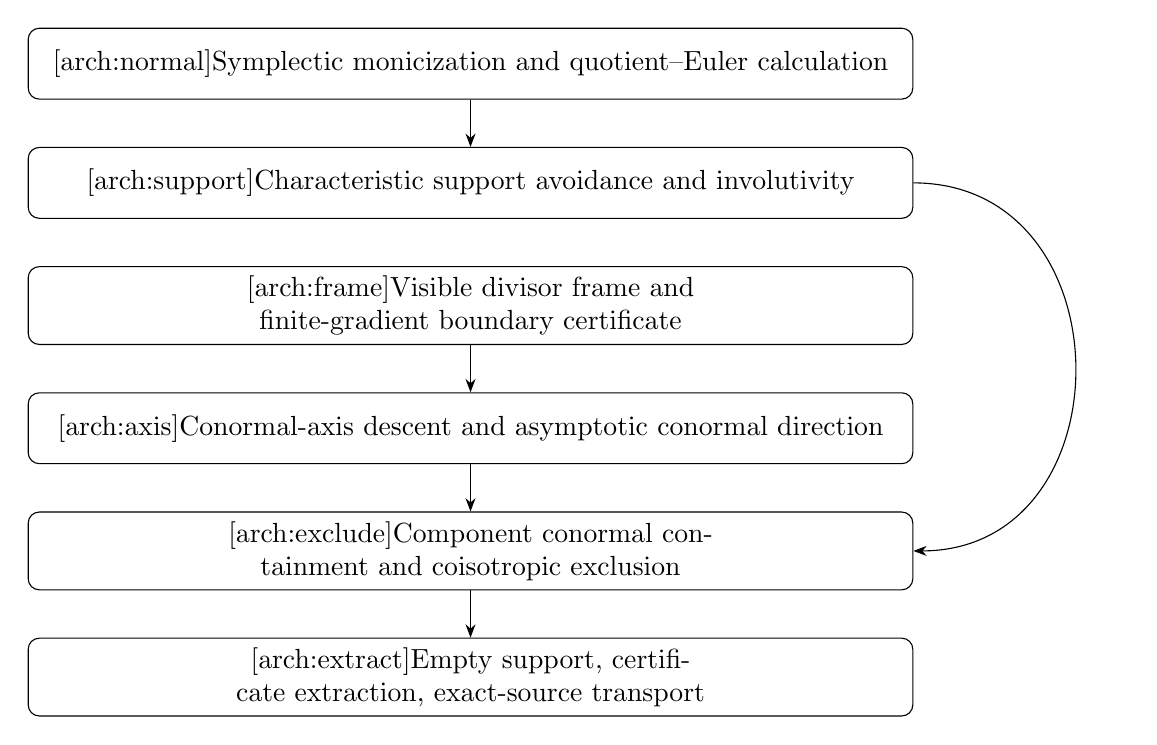
\begin{tikzpicture}[node distance=6mm,
 box/.style={draw,rounded corners,text width=11cm,align=center,minimum height=9mm},
 edge/.style={-{Stealth}}]
\node[box] (a) {\hyperref[arch:normal]{Symplectic monicization and quotient--Euler calculation}};
\node[box,below=of a] (b) {\hyperref[arch:support]{Characteristic support avoidance and involutivity}};
\node[box,below=of b] (c) {\hyperref[arch:frame]{Visible divisor frame and finite-gradient boundary certificate}};
\node[box,below=of c] (d) {\hyperref[arch:axis]{Conormal-axis descent and asymptotic conormal direction}};
\node[box,below=of d] (e) {\hyperref[arch:exclude]{Component conormal containment and coisotropic exclusion}};
\node[box,below=of e] (f) {\hyperref[arch:extract]{Empty support, certificate extraction, exact-source transport}};
\draw[edge] (a)--(b);
\draw[edge] (c)--(d);
\draw[edge] (b.east) to[out=0,in=0,looseness=1.5] (e.east);
\draw[edge] (d)--(e);
\draw[edge] (e)--(f);
\end{tikzpicture}
\end{center}

\subsection{Normalization}\label{arch:normal}
An invertible linear symplectic change makes the selected coordinate monic
with exponent equal to the Bernstein degree. The quotient--Euler calculation
retains the original operator as the right divisor in the second generator.
See \file{Stafford38/Weyl/MonicNormalization.lean} and
\file{Stafford38/Weyl/EulerRemainder.lean}.

\subsection{Support}\label{arch:support}
The canonical Koszul argument gives characteristic support avoidance.
\file{Stafford38/Characteristic/GabberGlobalAssembly.lean} proves involutivity
of the radical graded annihilator. Both feed the canonical coisotropic
application in \file{Stafford38/Geometry/GeneralCoisotropicCanonicalAdapter.lean}.

\subsection{Visible frame}\label{arch:frame}
In the transcendental-coordinate branch,
\file{Stafford38/Geometry/GeneralConormalAxis.lean} obtains a normalized
compatible visible divisor frame from
\file{Stafford38/Geometry/GeneralDivisorialVisibleFrame.lean}, which is built
on the retained-valuation data of
\file{Stafford38/Geometry/ExactDivisorialVisibleFrameExistence.lean} and the
generic divisorial frame construction of
\file{Stafford38/Geometry/DivisorialVisibleFrameStageAssembly.lean}. It then
applies the finite-gradient boundary certificate of
\file{Stafford38/Geometry/FiniteGradientResidueExtension.lean}. This is the
imported route; the earlier proof account cited the separately proved
tangent-limit lemma here, which this route does not import.

\subsection{Axis and descent}\label{arch:axis}
The certificate gives a conormal axis over the ground field.
\file{Stafford38/Geometry/GeneralAsymptoticLaurentAxis.lean} combines this
with the separate algebraic-coordinate branch. Smooth-fibre vanishing and
scalar-extension descent yield the projective conormal direction in
\file{Stafford38/Geometry/GeneralAsymptoticConormal.lean}.

\subsection{Exclusion}\label{arch:exclude}
\file{Stafford38/Geometry/GeneralComponentConormalContainment.lean} supplies
the component containment step. Together with asymptotic conormal geometry it
gives the coisotropic exclusion theorem
(\file{Stafford38/Geometry/GeneralCoisotropicExclusion.lean},
\file{Stafford38/Geometry/GeneralCoisotropicSets.lean}), which makes the
canonical support empty.

\subsection{Extraction}\label{arch:extract}
Certificate extraction and the inverse symplectic change give
$1=dR+\ell^{\deg_Bd}dS$ in the written order. The exact-source Challenge
transport proves equality of the intrinsic filtration degree and the PBW
normal-form degree; it does not merely restate an arbitrary-$F$ result.

\section{How the pairs are checked}

\VerbatimInput[fontsize=\small,frame=single,label=comparator.json]{\srcroot/comparator.json}

Comparator exports the compared theorem
(\file{Stafford38Challenge.universalStatement} for the original pair,
\file{Stafford38FixedSourceChallenge.universalFixedSourceStatement} for the
exact-source pair) from the challenge and solution environments separately,
checks that the two statements agree, checks that the solution's proof uses
only \lean{propext}, \lean{Quot.sound} and \lean{Classical.choice}, and
submits the exported proof to NanoDa and to Lean's own kernel. Each
challenge's transitive import closure is checked to contain only Lean core
and the pinned Mathlib; each solution's closure is checked not to contain
either challenge.

Both compared pairs passed Comparator, NanoDa and Lean kernel checking at
source commit \lean{cbb2396d}. The controller-host verifier also passed all
20 endpoint and 14 consumer reports. The original pair remains unchanged;
the exact-source pair exposes the stronger manuscript conclusion.

\begin{center}
\begin{tabular}{@{}p{5.2cm}l@{}}
\toprule
Repository & \lean{itpplasma/stafford38-formal} \\
Lean & \lean{leanprover/lean4:v4.33.0} \\
Mathlib & \lean{db584cd6d46c92f209a44c0f1c829460d327499d} \\
AlgebraicAnalysis \lean{v0.3.0}, public dependency of the solutions from \lean{v1.1.0} & \lean{4aae47967f6ba02ffe2f639ab06564c9a9d1ecc8} \\
AlgebraicAnalysis \lean{v0.2.0}, in the recorded \lean{v1.0.2} run & \lean{dfdd2da091a9d67e7a29cc7914f192d746a2400d} \\
Comparator / lean4export / NanoDa & \lean{5756749} / \lean{15f6055} / \lean{68d5ca9} \\
Permitted axioms & \lean{propext}, \lean{Quot.sound}, \lean{Classical.choice} \\
\bottomrule
\end{tabular}
\end{center}

\begin{sloppypar}
The source commit and machine-readable evidence are in
\lean{docs/verification-results.json}. This release records controller-host
checks. A separate isolated public-clone replay and human expert review are
not claimed. The author authorized publication before that additional replay.
\end{sloppypar}

\section{Literature and proof sources}\label{sec:literature}
Documentation release v1.1.1, 9 September 2026. Mathematical declarations and dependency pins are unchanged.

The conjecture node refers to \cite{Sta78}. The involutivity node implements
the classical theorem \cite{Gab81}; characteristic varieties have the background
\cite{HTT08}. Ore division has the ancestry \cite{Ore33}. The Euler certificate
and visible-frame/finite-gradient route are project constructions. The
auxiliary tangent-limit theorem is outside that terminal route. The survey
\cite{Bel26} and constructive work \cite{Ley04} give historical context.

Full source roles and clickable Lean entry points are indexed at \url{https://github.com/itpplasma/stafford38-formal/blob/main/docs/literature.md}.

\begin{thebibliography}{StacksS}
\bibitem[Sta78]{Sta78} J. T. Stafford, \emph{Module Structure of Weyl Algebras}, Journal of the London Mathematical Society (2) 18 (1978), 429–442. \url{https://doi.org/10.1112/jlms/s2-18.3.429}.
\bibitem[Gab81]{Gab81} Ofer Gabber, \emph{The Integrability of the Characteristic Variety}, American Journal of Mathematics 103 (1981), no. 3, 445–468. \url{https://doi.org/10.2307/2374101}.
\bibitem[HTT08]{HTT08} Ryoshi Hotta, Kiyoshi Takeuchi, and Toshiyuki Tanisaki, \emph{D-Modules, Perverse Sheaves, and Representation Theory}, Progress in Mathematics 236, Birkhäuser, 2008. \url{https://doi.org/10.1007/978-0-8176-4523-6}.
\bibitem[Ore33]{Ore33} {\O}ystein Ore, \emph{Theory of Non-Commutative Polynomials}, Annals of Mathematics (2) 34 (1933), no. 3, 480–508. \url{https://doi.org/10.2307/1968173}.
\bibitem[StacksD]{StacksD} The Stacks Project Authors, \emph{Finite order differential operators}, The Stacks Project, Section 10.133, tag 09CH (accessed 2026-09-09). \url{https://stacks.math.columbia.edu/tag/09CH}.
\bibitem[Bel26]{Bel26} Gwyn Bellamy, \emph{Module structure of Weyl algebras}, Journal of the London Mathematical Society 113 (2026), no. 1, e70373. \url{https://doi.org/10.1112/jlms.70373}.
\bibitem[Ley04]{Ley04} Anton Leykin, \emph{Algorithmic Proofs of Two Theorems of Stafford}, Journal of Symbolic Computation 38 (2004), 1535–1550. \url{https://doi.org/10.1016/j.jsc.2004.07.003}.
\end{thebibliography}
\end{document}
